\chapter{The UAV control problem}\label{ch:UAVControlProblem}

%1.1 The control problem
%Focus on the key idea of conciliating optimal trajectories in order to improve performance of the system with avoidance of collision with obstacles, and, then dwell on the overall approach:
%a) The model predictive control scheme a a recursive technique to approximate optimal trajectories.
%Include a MPC scheme here.
%b) Type of sensory data and its processing
%c) Obstacle Avoidance
%d) Control switch strategy
%e) Low level control
%Include here the Control Architecture diagram below.

%1.2 Assumptions that play a key role in the problem formulation.
%(if you do not detail this a lot (as it is now), you may suppress the sections in this chapter)

\noindent This chapter specifies Model Predictive Control (MPC) architecture for UAV and defines assumptions.
\section{The control problem}
\noindent \textit{Obstacle avoidance} in terms of control is complex optimisation problem with dynamic constraints. This works addresses know obstacles only, therefore MPC generates semi-optimal control sequence. Movement constraints are mainly given by static uncharted obstacles and non-cooperative intruders. This work focus on charted obstacles. Uncharted obstacles and non-cooperative intruders are omitted in this work. Model Predictive Control is established for optimal trajectory calculation and reach set $\mathscr{R}$ estimation. Constraints in terms of obstacle discovery are relaxed. Usually multiple layer control concept is used. Control concept used for this work is in fig. \ref{fig:controlConceptIntro}.
\begin{figure}[H]
    \centering
    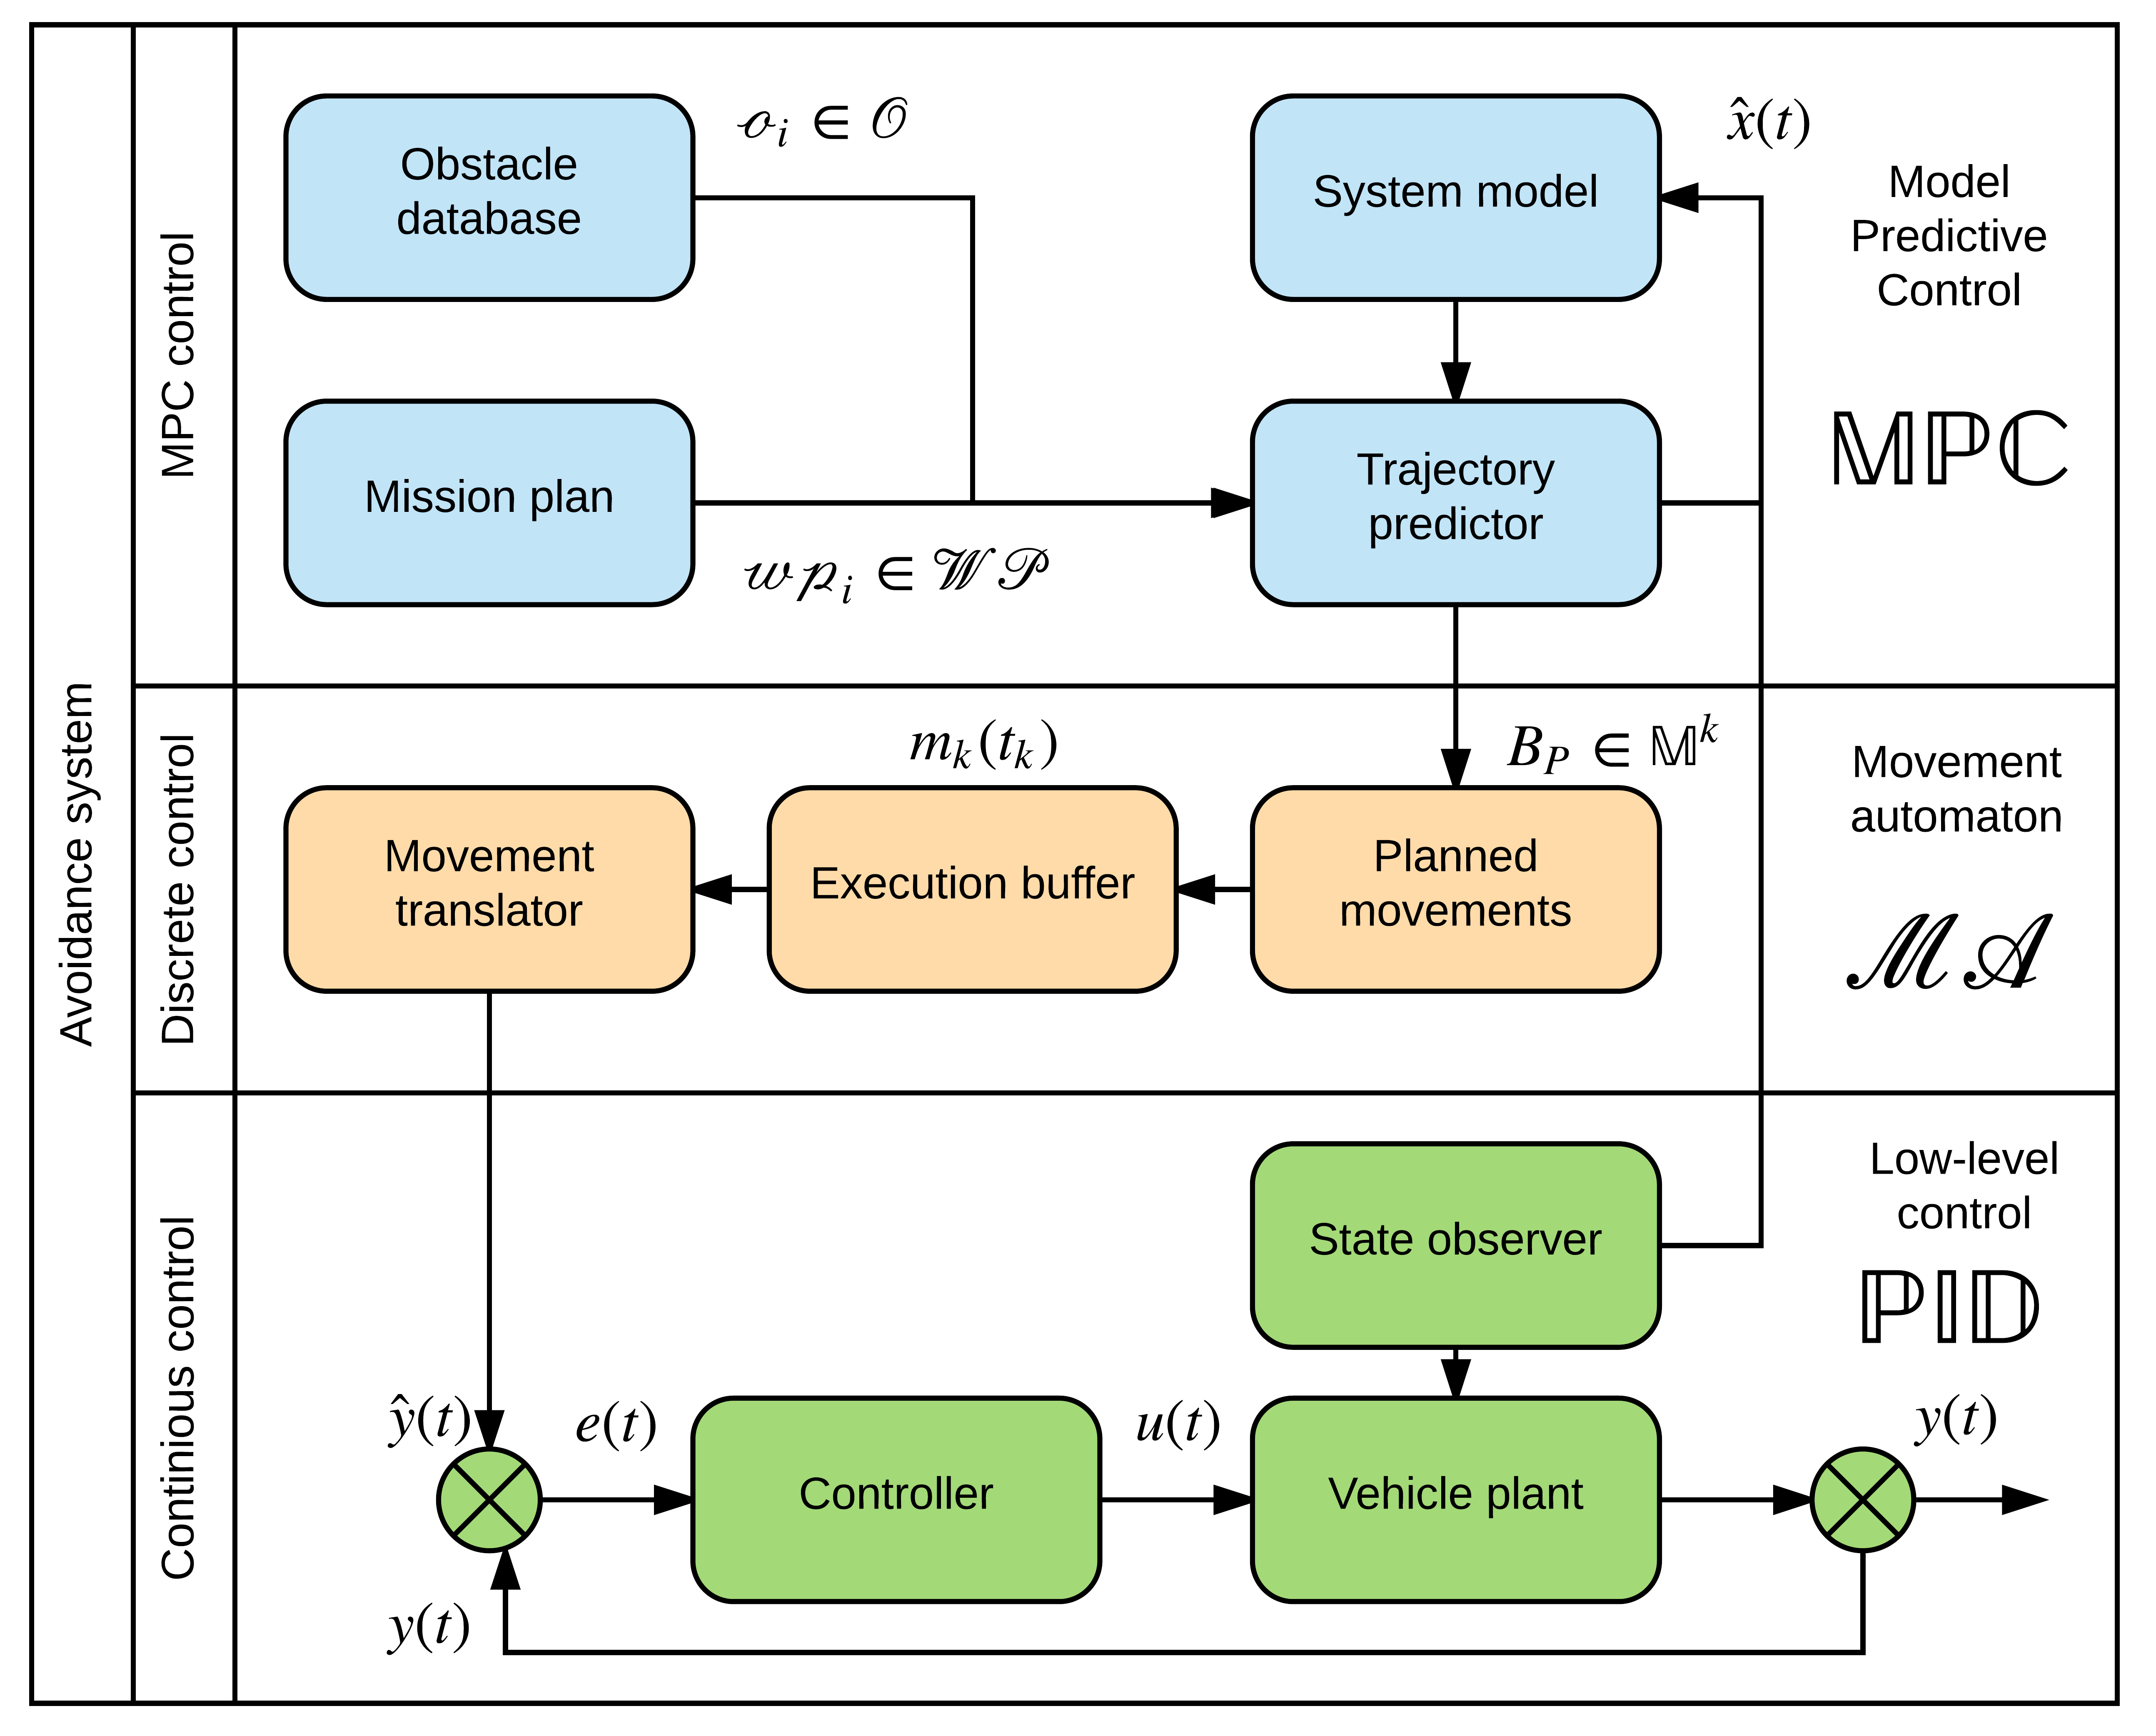
\includegraphics[width=.75\linewidth]{\FIGDIR/72_Control_Concept.png}
    \caption{Control concept for MPC with $\mathscr{MA}$.}
    \label{fig:controlConceptIntro}
\end{figure}

\noindent \textit{Event based control} module is responsible for abstract level decisions and mission execution. This module generates abstract level input commands which are optimal to given criterion. MPC in this case is taken into event base level. MPC in this work is triggered by consumption of of all movements in movement automaton $\mathscr{MA}$ buffer $B$. There is no re-planning trigger due to trajectory deviation from original estimation. The reason is that system model and Vehicle plant are using same model in simulation (in nonlinear form and in linearized form for predictor)  \textit{Event based control} consist from following components:
\begin{enumerate}
    \item \textit{Obstacle database} - provides relevant obstacle data for trajectory planning, contains obstacle set $\mathscr{O}$ with obstacle records $o_i$. This module is data provider. Sensor fusion is omitted in this work.
    \item \textit{Mission plan} - contains mission plan $\mathscr{WP}$, determines navigation goal waypoint $\mathscr{WP}_g$.
    \item \textit{Trajectory predictor} - produces movement chain $B_p\in \mathbb{M}$. This module represents Model predictive control. It is using \textit{System model} to predict future states in finite prediction window. This module predicts trajectory between each waypoint $w_i,w_{i+1}\in\mathscr{WP}$. Prediction is invoked at time of decision $t_d$. Predictor then uses \textit{System model} with initial state $\hat{x}(t_d)$ form \textit{State observer} module. Predictor calculates optimal trajectory to avoid obstacles in obstacle set $\mathscr{O}$ and reach waypoint $w_{i+1}$.
    \item \textit{System model} - interprets system dynamics response to movement chain $m_1(t_1),\dots,m_i,t_i$ with initial state $x(t_0)=\hat{x}(t_{d_{i-1}})$. This module is mainly used to predict feasible trajectories around known obstacles set $\mathscr{O}$. \textit{System model} have been implemented as linear state predictor, because of system dynamics. Computation light techniques should be preferred in case of other non-linearizable systems. 
\end{enumerate}

\noindent \textit{Discrete control} module is responsible for processing abstract level movement command chain $B_p \in \mathbb{M}^k$. It is implemented as special type of open hybrid automaton, movement automaton $\mathscr{MA}$. Movement automaton $\mathscr{MA}$ have following notable modules:
\begin{enumerate}
    \item \textit{Planned movements} - buffers planned movements from avoidance grid $B_P\in\mathbb{M}^k$, planed movements buffer can be extended by additional movements (normal situation) or filled with new movement chain(flush) in case of trajectory correction or avoidance. Planned movement is similar to FIFO stack.
    \item \textit{Execution buffer} - executes first command from \textit{planned movements}, based on previous movement $m_{k-1}(t_{(k-1)})$ and actual command $m_k(t_k)$ chain of movement primitives $\{p_1, \dots p_l\}$ is created. Chain of movement primitives $\{p_1, \dots p_l\}$ is forwarded to movement translator (mapping module).
    \item \textit{Movement translator} - maps chain of movement primitives or other movement representation to:
    \begin{enumerate}[a.]
        \item \textit{Desired input signal $\hat{u}(t)$,} - in case of \textit{open loop control}, in this case desired control signal is feed directly to \textit{controlled plant}.
        \item \textit{Desired output signal $\hat{y}(t),t\in<t_{(k-1)},t_k)$} - in case of \textit{closed loop control}, in this case desired output signal is feed to closed loop controller. If there is closed loop controller, there is possibility for low level optimisation of control.
    \end{enumerate}
\end{enumerate}

\noindent \textit{Continuous control} module is target for low level control optimisation techniques. It is expected that \textit{controlled plant} is observable at least at position and orientation state parameters. \textit{State observer} provides observed state within critical time frame. \textit{Continuous control} module is responsible for low level control of plant with following modules:
\begin{enumerate}
    \item \textit{Control} - standard closed loop control component, using error $e(t)$ as input and actuating unit signal $u(t)$ as output.
    \item \textit{Controlled plant} - controlled vehicle plant, can be subsurface marine vehicle or aerial vehicle
    \item \textit{State observer} - observing state of controlled plant $\hat{x}(t)$.
\end{enumerate}

\subsection*{Trajectory prediction technique}
\noindent \textit{Trajectory} is constrained by set of waypoints $\mathscr{WP}$ and set of obstacles $\mathscr{O}$. Obstacle set $\mathscr{O}$ is constant. \textit{Trajectory search} in static environment is problem which needs to address following concurrent requirements:
\begin{enumerate}
    \item \textit{Calculation time} - avoidance trajectory calculation time must be shortest possible to assure optimal \textit{prediction window}.
    \item \textit{Estimation precision} - avoidance trajectory estimation must be precise enough to guarantee safety of predicted trajectory. Predicted trajectory with some estimation error, should not lead to vehicle crash. 
    \item \textit{Estimation optimality} - predicted trajectory should minimize optimality criterion or cost function $J(\circ)$.
\end{enumerate}
\noindent In case of \textit{Estimation optimality} requirement, only known world is taken into account. For real \textit{Estimation optimality} all obstacles static or dynamic needs to be known at time of prediction. This constraint is not guaranteed in future obstacle avoidance system. This work consider all obstacles to be known prior the flight. This requirement can be reduced to \textit{Estimation sub-optimality}.

Model predictive control gives discrete time optimisation technique to be used used on obstacle avoidance \textit{event based control} level.  Continuous optimisation techniques to increase movement automaton $\mathscr{MA}$ execution precision can be used in \textit{closed loop control}. Chosen optimisation techniques for movement chain optimisation is \textit{rapid exploration tree}. This prediction technique is not trivial search technique and it demonstrates qualities of discrete time optimum search.

\subsection*{Type of sensory data and its processing}
\noindent In future solution \textit{LiDAR is main sensor}. There is planned addition for \textit{ADS-B} transceiver /receiver for moving cooperative obstacle Sense \& Avoid. LiDAR data will be represented as positional vector $\vec{p}=[d,\theta,\varphi]$, where $d$ is distance to point, $\theta$ is horizontal offset angle and $\varphi$ is vertical offset angle in local coordinates frame. Only one matter point $\vec{p}$ is scanned at given scanning time $t_s$, in case of LiDAR sensor with one active scanner. 

LiDAR data for one LiDAR sweep at time interval $(t_s, t_e] $are given as series of points and scanning time pairs $\left\{\{\vec{p}_1\,t_s\},\{\vec{p}_2,t_2\},\dots,\{\vec{p}_n,t_e\}\right\}$. These points needs to be normalized at time $t_e$ in \textit{local coordinate frame} with center at vehicle position $[x_v,y_v,z_v]$ and rotated by vehicle orientation $[-\alpha_v,-\beta_v,-\gamma_v]$. One LiDAR sweep covers area given by scanning distance $[d_s,d_e]$, horizontal range $[\theta_s,\theta_e]$ and vertical range $[\varphi_s,\varphi_e]$. One LiDAR sweep covers rectangular conical cut in front of the scanning vehicle. All mission $\mathscr{WP}$ area and obstacle set $\mathscr{O}$ is know prior the mission execution.

For global coordinates Earth geocentric reference model \textit{WGS-84} is used, therefore \textit{GPS} is considered as main source of position. In later stages mixed position mode using \textit{GLONASS} system can be incorporated. \textit{GLONASS} is using \textit{PG-90} reference model. Transformation between \textit{PG-90} and \textit{WGS-84} are mentioned in \cite{misra1996integrated}. For further mentions of \textit{global coordinate frame} reference frame \textit{WGS-84} is always used.

\textit{Obstacle map} is using global coordinate frame, where obstacles are represented by center of their mass $\vec{p}_c$ and protective range $r$. Obstacle body is then given by unit ball around $\mathscr{B}(\vec{p}_c,r)$.

\noindent\textit{Sensor fusion} is fusing following data sources in local coordinate frame of vehicle:
\begin{enumerate}
    \item \textit{LiDAR sensor sweep (planned)} - based on LiDAR sensor reading point-cloud in front of vehicle is filtered by Extended Kalman Filter \cite{blanc2005ekf}. Visibility space is then partitioned into \textit{free, obstacle} and \textit{uncertain} subspaces.
    \item \textit{Obstacle map (planned)} - based on known obstacle map, the obstacles in Field Of Vision range are selected and fused into vehicle`s local coordinate frame. Free space previously unoccupied by by obstacles is marked as \textit{map obstacle occupied}.
    \item \textit{Intruders (planned)} - based on ADS-B reading and LiDAR data processing moving cooperative and non-cooperative intruders are identified. Portions of free space occupied by intruders in expected reach time are then marked as \textit{intruder occupied}.
\end{enumerate}

\noindent Result of future \textit{sensor fusion} will be used as base for \textit{Trajectory predictor}.

\subsection*{Obstacle avoidance}
\noindent \textit{Obstacle avoidance} is continuous process which is triggered by waypoint change. When \textit{Control strategy switch} changes mode to another waypoint following steps are executed until the reaching next waypoint:
\begin{enumerate}
    \item \textit{Next movement selection} - main contributor is \textit{Obstacle database}. \textit{Trajectory predictor} calculates critical distance to relevant obstacles $o_i\in\hat{\mathscr{O}}(t_{i-1})$ in predicted state $\hat{x}(t_i)$ after application of movement $m_i(t_i)$. Estimated obstacle set $\hat{\mathscr{O}}(t_i)$ is calculated after predicted movement execution.
    \item \textit{Feasibility assessment} - predicted movement state $\hat{x}(t_i)$ is compared to estimated obstacle set $\hat{\mathscr{O}}(t_i)$. If there is no approaching danger, movement is added to planned movements $B_p$ and next movement for $t_i=t_{i+1}$ is executed. If there is approaching danger systems use backtracking approach to determine feasible movements. If more than one movement is re-planned, then movement chain is changed according to new estimated movement chain.
\end{enumerate}
\noindent This approach is similar to \textit{Dynamic programming} backtracking.

\noindent Avoidance trajectory $\mathscr{T}(\vec{x}_i,t_i)$ generated for state $\vec{x}_i$ at decision time $t_i$. Executed movement buffer is given by chained prediction frames $\mathscr{P}(w_p)$. frames as  $\mathscr{T}= \cup_{i=\{wp_1,\dots,wp_n\}} \mathscr{T}(\vec{\hat{x}}_{wp_i},t_{wp_i})$ is optimal in known world \cite{kochenderfer2008encounter}.

\subsection*{Low level control}
\noindent \textit{Low level control} must be decoupled in order to implement movement automaton $\mathscr{MA}$. Various decoupling methods tor under-steered systems (less inputs than controlled variables) can be used, for example \cite{das2009dynamic}.

\section{Assumptions}
\noindent
The following assumptions are considered in this work:
\begin{assumption}{There is relevant obstacle database and no other static obstacles exists during a mission execution}\label{ass:1}\end{assumption}
\noindent Point-cloud is main source of constraints and obstacles. Main constraint is terrain and charted obstacles. Vehicle has discovered world prior the flight.  

\begin{assumption}{There are no moving obstacles.}\label{ass:3}\end{assumption}
\noindent This condition will be later relaxed after full \textit{sensor fusion} implementation.

\begin{assumption}{Estimates of the state of the UAV are available.}\label{ass:4}\end{assumption}
\noindent This condition is can be interpreted in way, that \textit{State observer} module can observe vehicle position $[x_v,y_v,z_v]$ and orientation $[\alpha_v,\beta_v,\gamma_v]$ in real time. 

\begin{assumption}{The operational space does not contain 'traps' such as caves. 'Traps' arise because the field of view of the LiDAR does not include the whole space surrounding the UAV.}\label{ass:5}\end{assumption}
\noindent \textit{Convex traps} can not be addressed by this approach, due the insufficient rules in \textit{Rule engine} module. When \textit{convex trap} avoidance rules will be implemented into rule engine it will be possible to relax this assumption.

\begin{assumption}{There is a mission plan for the UAV consisting of waypoints.} \label{ass:6} \end{assumption}

\noindent Trajectory given by mission plan is not optimal, because it is just joint lines between waypoints. Dynamic of most system does not allow to follow this type of route, therefore route considering reach set of vehicle $\mathscr{R}$ needs to be calculated prior the mission execution or \textit{Trajectory predictor} is used as route planning tool. 